%-----------------------------------------------------------------------------
%
%               Thrudb white paper
%
% Name:         thrudb.tex
%
% Authors:      T Jake Luciani (jake@3.rdrail.net)
%
% Created:      25 October 2007
%
%-----------------------------------------------------------------------------


\documentclass[nocopyrightspace,blockstyle]{sigplanconf}

\usepackage{amssymb}
\usepackage{amsfonts}
\usepackage{amsmath}
\usepackage{url}
\usepackage{graphicx}

\begin{document}

% \conferenceinfo{WXYZ '05}{date, City.} 
% \copyrightyear{2007}
% \copyrightdata{[to be supplied]} 

% \titlebanner{banner above paper title}        % These are ignored unless
% \preprintfooter{short description of paper}   % 'preprint' option specified.

\title{Thrudb: Document Oriented Database Services}
\subtitle{}

\authorinfo{T Jake Luciani}
	   {http://thrudb.googlecode.com | http://3.rdrail.net}
           {jake [at] 3.rdrail.net}
\maketitle

\begin{abstract}
Thrudb is a set of simple services built on top of Facebook’s Thrift framework that provides 
indexing and document storage services for building and scaling websites. 
It’s purpose is to offer web developers flexible, fast and easy-to-use services that can 
enhance or replace traditional data storage and access layers.
   
This paper explains the services thrudb provides as well as the underlying libraries and choices 
made when designing it.  Note, this is not an actual research paper, but it looks more impressive 
when styled as one.
\end{abstract}

%\category{D.3.3}{Databases}{Services}

%\terms
%Database, storage, indexing, service

%\keywords
%Data storage, information retrieval, web development

\section{Introduction}
Relational databases are the backbone of modern websites.  Along with web servers, they enable the 
world wide web by allowing anyone with a web browser to extract and interact with data and documents.  
The traditional LAMP stack has provided everything needed to build websites, but with the onset of web 2.0
there are numerous programming frameworks and web services that can simplify the development effort. 
As well as countless techniques and enhancements to improve the speed and scalability of your site once deployed.

There is still one area that is difficult to design and deploy correctly however, the data layer.
 
Data on the web is often fluid and loosely structured and it is becoming increasingly difficult to fit into a fixed database schema which is amend over time.
A simple example of this is tagging. The many to many relationship of tags are difficult to query efficiently using tables and SQL requiring ad-hoc solutions.

Also, Web data is often "mashed up" and viewed together (facebook profile) or viewed spatially (google maps + event data). 

In order to provide this new kind of data flexibility the web is moving towards a document oriented data model.  Where records arena't grouped by their structure but by their attributes.  

Object relational mapping libraries (Hibernate, Active Record) attempt to hide the underlying relational model but the fact remains sparse and unnormalized data was not intended for these systems. 

There are also standard data oriented issues like indexing, caching, replication and backups, which are left for "later" but are never easy to employ when its time to do it.
There are a number great of open source components that currently provide solutions to these problems but they require proper integration and configuration.  These components end up being picked over time by learned by trial and error.

Thrudb, therefore, is an attempt to simplify the modern web data layer and provide the features and tools most web-developers need that can be easily configured or turned off.

It can be used on traditional hosting setups but is also intended to be deployed on Amazon's EC2 using Amazon S3 as it's storage backend.

When designing Thrudb the following requirements were identified:

\begin{itemize}

\item\textit{Modular.} Each service should be valuable on its own and impose no requirements on the others.

\item\textit{Simple.} The APIs must be obvious and work in most languages.

\item\textit{Fast.} The services must be written in a compiled language, be multi-threaded when necessary and use asynchronous processing when necessary.

\item\textit{Flexible.} The services should be capable of handling any type of document you can throw at it. 

\item\textit{Easy to manage.} The configuration of these services should be simple and fairly obvious. no sendmail.cf 

\item\textit{Redundant.} The data should be replicatable and provide multi-mastership writes

\item\textit{Recoverable.} The services should be ACID compliant and provide redo logs and incremental backups

\item\textit{Scalable.} The system should be horizontally scalable and provide write-through caching  
\end{itemize}

What came out the other end were the following services:

\begin{itemize}
\item\textit{Thrudoc}   - Document storage service. See Section 2. 

\item\textit{Thrucene}  - Document indexing service. See section 3.

\item\textit{Throxy}    - Service proxy and partition aggregator. See section 4.
\end{itemize}

These services are built with the help of the following open source projects:
\begin{itemize}
\item\textit{Thrift}    - Facebook's framework for providing cross-language services.  This is the backbone of Thrudb. \footnote{See http://developers.facebook.com/thrift}

\item\textit{Lucene}    - Specifically CLucene, which provides high performance indexing. \footnote{See http://clucene.sf.net}

\item\textit{Spread}    - Guaranteed messaging bus with reliable membership updates. \footnote{See http://spread.org}

\item\textit{Amazon Services} -Not open source but almost free scalable computing and storage platform. \footnote{See http://www.amazonaws.com}

\item\textit{memcached} - Highly scalable distributed caching service. \footnote{See http://danga.com/thrift}

\item\textit{brackup}   - Nifty backups to disk or S3. \footnote{See http://search.cpan.org/~bradfitz/Brackup-1.06/brackup}
\end{itemize}

\section{Thrudoc}

Thrudoc is a simple key value storage system designed to work on a number of underlying storage backends, such as files on disk or S3 records.
Its purpose is to provide simple scalable access to any stored object.

Let's start with a simple example in perl: 

\begin{verbatim}
######################################################
my $socket    = new Thrift::Socket('localhost',9091);
my $transport = new Thrift::FramedTransport($socket);
my $protocol  = new Thrift::BinaryProtocol($transport);
my $client    = new ThrudocClient($protocol);

$transport->open();

my $id = $client->store("a serialized doc");
  
print "Recieved: ".$client->fetch($id);

$client->store("an updated doc",$id);

$client->remove($id);

\end{verbatim}
  
Since thrudb is built on top of thrift this client API is available naively in most languages.
The \textit{value} parameter can be a string, json object, xml object, or a serialized thrift object.

We recommend Thrift objects because they support structure visioning.  

Briefly, this means if your website launches and you forgot to include "address" in the user 
structure but already have thousands of users you don't re-create your old objects. Simply add the address field
to your Thrift object definition it will support both old and new versions of your serialized object. 
\footnote{See Appendix A for a further discussion on thrift objects.}

Thrudb's identifiers are by default UUIDs. This removes the dependency on centralized or incremental identifiers (not scalable).
You can specify a key identifier of your own but a new id will be returned that is the MD5 value of the key. 
This keeps the storage area balanced. 

Also note, there is no concept of different storage locations, everything is stored together in what appears to be one big bucket.

Thrudb supports multiple storage backends.  Initially these include local disk storage or S3 but this could be easily extended. 

Thrudb also offers caching, partitioning, replication with multi-master writes, redo logs and backups. Each of these 
will be described later in this document.

\section{Thrucene}

Thrucene exposes the Lucene Search API as a Thrift service.  

Its purpose is to provide powerful searching capabilities for your documents.  
This is intended to be used with the Thrudoc service but can be used to provide search for traditional database records as well. 

The idea of your index living separately from your document isn't new.  
Google is built this way since an index store can scale very differently then your documents document store.  
For example, you may only be interested in searching a few fields within your documents or
wish keep multiple indexes on the same set of documents. This is similar to MapReduce
\footnote{See http://code.google.com/edu/parallel/mapreduce-tutorial.html}

Hence, with Thrucene you can create multiple indexes and use them to search any relevant information about your documents.

You can rebuild a complete index from a document store or you can incrementally update your 
index as you update your documents to simulate a traditional database layer.

Heres a simple example:

\begin{verbatim}
#############################################
#Create a bookmark
my $b = new Bookmark(); #thrift obj

$b->name("Thrudb: Document Services");
$b->url("http://thrudoc.googlecode.com");
$b->tags("database thrift web2.0");

my $bm_id = $thrudoc->store( $b->write() );
  
#############################################
#Index it
my $d = new Thrucene::DocMsg();

$d->domain( "tests"      );
$d->index (  "bookmarks" );
$d->docid ( $bm_id       );

my $field = new Thrucene::Field();

$field->name( "tags" );
$field->value( $b->tags );

push(@{$d->{fields}}, $field);

$thrucene->add( $d );
$thrucene->commitAll();

\end{verbatim}

In this example we created a bookmark and indexed it, now we'll show how to search bookmarks.
\footnote{See http://lucene.apache.org/java/docs/queryparsersyntax.html for query syntax}

\begin{verbatim}
#########################################
#Find some bookmarks
my $q = new Thrucene::QueryMsg();

$q->domain( "test" );
$q->index ( "bookmarks" );
$q->query ( "tags:(+database +web2.0)" );
   
my $r = $thrucene->query( $q );

print "Found documents".join(",",@{$r->{ids}});

\end{verbatim}

The query returns the matching document ids which can then be 
fetched from Thrudoc.

This service supports replication with multi-master writes, redo logging, partitioning, and backups.

Note, One great aspect of Thrucene is it's indexes can always be rebuilt from the document source. 
This allows us to comfortably deploy on Amazon's Compute Cloud using Thrudoc's S3 backend for 
document storage with no fear of data loss.   

\section{Throxy}

The Throxy service enables other thrudb services to be partitioned off and scaled horizontally.  
It sits between client and servers partitioning and aggregating writes and reads respectively.

This system is completely asynchronous and takes advantage of  
Thrift's distinct send and receive methods for each service call. 

Below is a diagram of all Thrudb services working together.

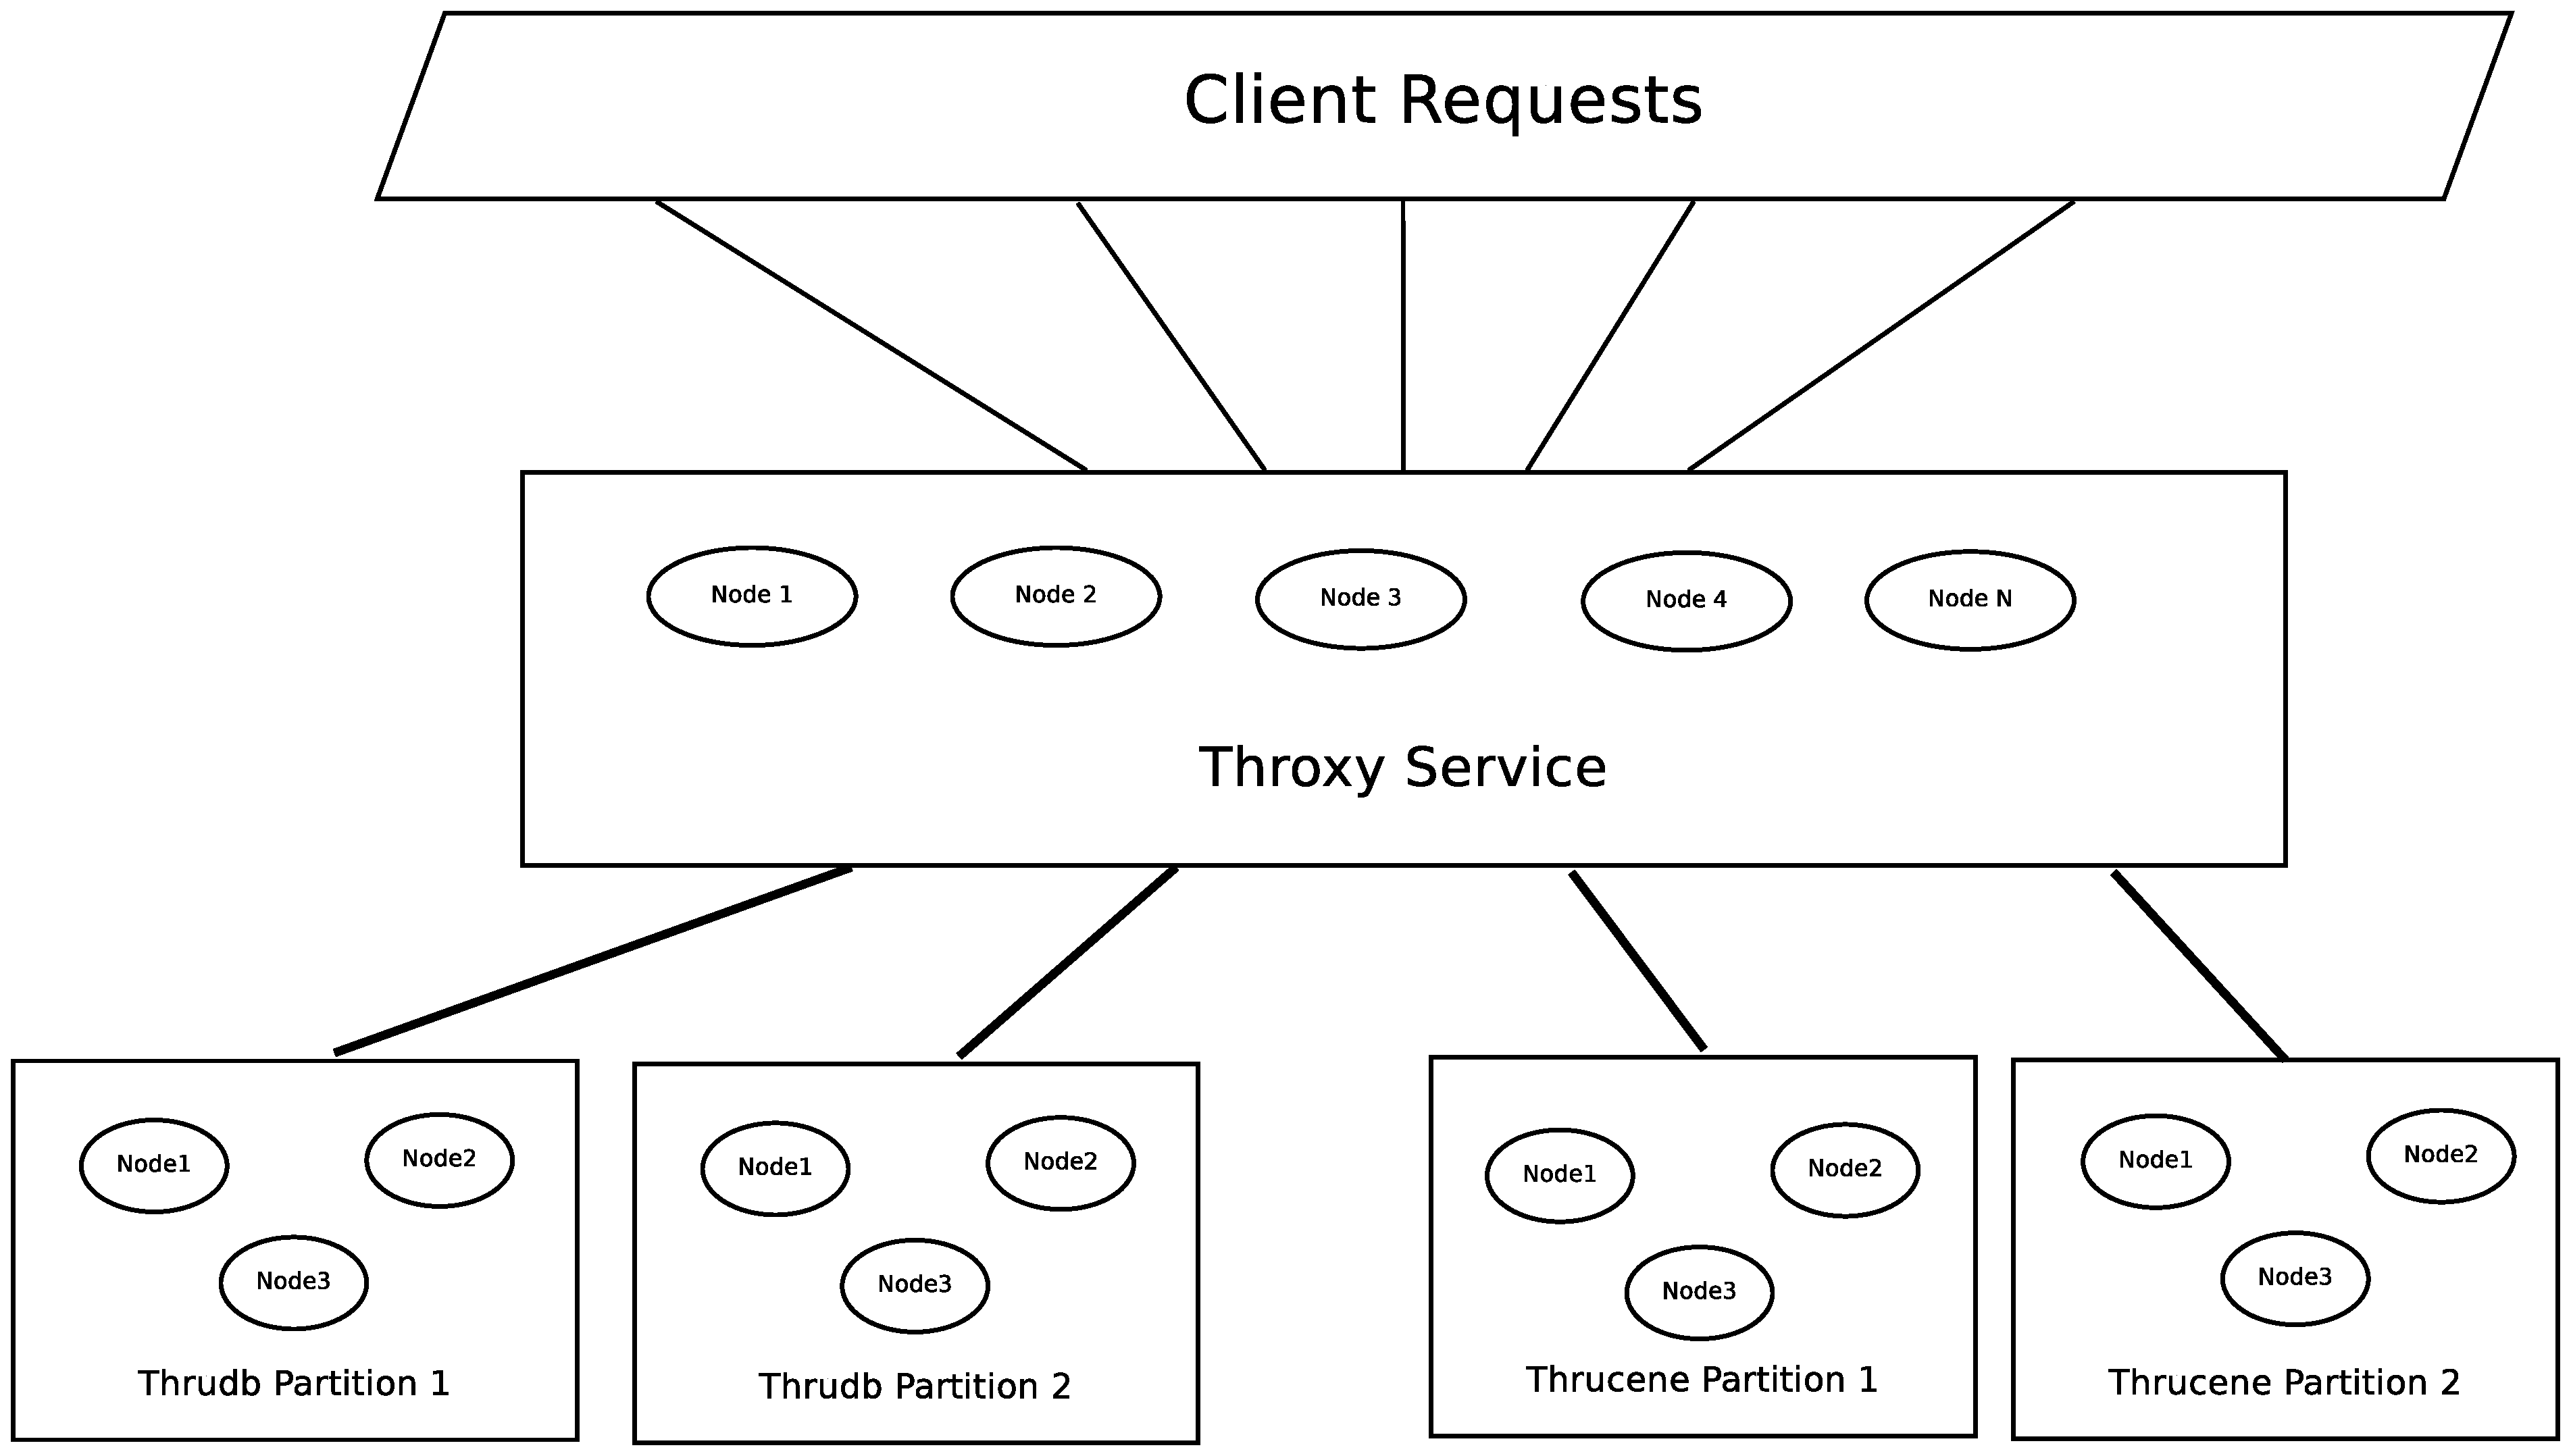
\includegraphics[width=3.00in]{Throxy.eps}

As mentioned earlier, all Thrudb services are optional. You can pick and choose the services and features you would like to integrate. 
By no means is this the required setup.

\section{Replication and Multi-Mastership}

Thrudoc and Thrucene both provide replication, for redundancy, and multi-master writes, for client simplicity, using 
Spread.  Spread was written to simplify building services that can synchronize with other instances to offer high availability.  

If Spread usage is enabled, your Thrudb services will communicate with each other via a Spread group and keep synchronized using two phased commits.

You define a Spread group to join and the minimum number of cohorts required for writes to succeed.  As usual, this can be turned off. 

The details of the communication protocol are outside the scope of this document. 

\section{Caching}

Thrudoc employs write-through caching of all documents. While Thrucene lets you cache particular queries.

The caching service is provided by Memcached.  

Memcached is well known as the best distributed caching service (period).  
It lets the client distribute documents across instances rather than try to maintain document locations itself. 
It also offers compression and great stability.
   
The memcached client used by Thrudb is intended to support multiple hashing algorithms for distributing documents around the cache.
Consistent hashing\footnote{See \url{http://en.wikipedia.org/wiki/Consistent_hashing}} is the recommended since it provides highest hit rate. 

Also, Memcached is currently used as the transport mechanism for replication as large documents would bog down Spread.

\section{Redo logging and Backup}

Redo logs are used for recovery purposes.  
For example, if you have three instances of Thrudoc replication in the same group and one instance goes down, when it comes back up, 
one of the other instances will replay it's redo log from the point the instance died to bring it back up to sync before it is
officially online.
  
Thrift has a built in file logging facility that makes it simple to create redo logs.

Complete backups of your documents or indicies are also taken systematically using Brackup\footnote{http://search.cpan.org/~bradfitz/Brackup-1.06/brackup}

Brackup has implemented a number of storage backends, but the backup tool itself is abstracted and can be swapped altogether with something else. 

\section{Appendix}

\subsection{Thrift}

To learn more about thrift please visit \url{http://developers.facebook.com/thrift}

\subsection{Bloom filters}

Thrudoc maintains a bloom filter\footnote{See \url{http://en.wikipedia.org/wiki/Bloom_filter}} 
for quickly detecting if a document exists in it's store.  
This becomes extremely important since reads affect performance and in the case of S3 you get charged for them.
This bloom filter can be recreated from the document source if corrupted.

\section{Thanks}

I'd like to thank the open source community for providing such great software.  
It has made an ambitious project like this something one person can accomplish.

I'd also like to thank Amazon web services for providing affordable and scalable
computing resources and storage.

\end{document}


